\documentclass[conference]{IEEEtran}
\usepackage{graphicx}
\usepackage{booktabs}
\usepackage{amsmath}
\usepackage{hyperref}
\usepackage{multirow}
\usepackage{float}

\title{MLOps Assignment 1: Deep Learning and SVM Classification on MNIST and FashionMNIST}
\author{\IEEEauthorblockN{Tejas Gupta}
\IEEEauthorblockA{B22CS093\\Indian Institute of Technology Jodhpur}}

\begin{document}
\maketitle

\begin{center}
\fbox{\parbox{0.95\columnwidth}{
\textbf{GitHub:} \url{https://github.com/TejasGupta-27/MLOps-TejasGupta-B22CS093}

\textbf{Kaggle Notebooks:}
\begin{itemize}
    \item Part 1: \url{https://www.kaggle.com/code/tejasgupta001/part1-mnist}
    \item Part 2: \url{https://www.kaggle.com/code/tejasgupta001/part2-fashionmnist}
    \item Part 3: \url{https://www.kaggle.com/code/tejasgupta001/part3-svm-cpu-gpu}
\end{itemize}
}}
\end{center}

\begin{abstract}
This report presents a comparative study of ResNet-18 and ResNet-50 on MNIST and FashionMNIST datasets, analyzing hyperparameter impact on classification accuracy. We evaluate the effects of batch size, optimizer choice, learning rate, epochs, and pin\_memory on model performance. Additionally, we compare SVM classifiers with deep learning approaches and analyze CPU vs GPU training efficiency. Our experiments achieve 99.12\% accuracy on MNIST and 90.67\% on FashionMNIST, with GPU providing up to 12x training speedup.
\end{abstract}

\section{Introduction}
Image classification serves as a fundamental benchmark for evaluating machine learning algorithms. This study systematically evaluates ResNet architectures and SVM classifiers on two widely-used datasets: MNIST (handwritten digits) and FashionMNIST (fashion items), with focus on hyperparameter sensitivity, computational efficiency, and practical deployment considerations.

\section{Methodology}
\textbf{Dataset Configuration:} 70-10-20 train-val-test split, images resized to 224$\times$224 for ResNet compatibility.

\textbf{Training Settings:} USE\_AMP=True (Mixed Precision), epochs $\in$ \{1,2\}, pin\_memory $\in$ \{True, False\}.

\textbf{Models:} ResNet-18 (11.7M params, 1.82B FLOPs), ResNet-50 (25.6M params, 4.13B FLOPs), SVM (poly/RBF kernels).

\section{Q1(a): Deep Learning Results}

\subsection{MNIST Results}
\begin{table}[h]
\centering
\caption{MNIST Test Accuracy (\%) - Best results per configuration (Epochs=2)}
\label{tab:mnist}
\begin{tabular}{cccccrr}
\toprule
BS & Opt & LR & Epochs & pin\_mem & ResNet-18 & ResNet-50 \\
\midrule
16 & SGD & 0.001 & 2 & True & 98.51 & 98.54 \\
16 & SGD & 0.001 & 2 & False & 98.73 & 98.67 \\
16 & SGD & 0.0001 & 2 & True & 95.16 & 92.43 \\
16 & SGD & 0.0001 & 2 & False & 92.21 & 90.38 \\
16 & Adam & 0.001 & 2 & True & 97.80 & 98.35 \\
16 & Adam & 0.001 & 2 & False & 98.65 & 98.44 \\
16 & Adam & 0.0001 & 2 & True & 98.91 & \textbf{99.06} \\
16 & Adam & 0.0001 & 2 & False & 98.80 & 98.70 \\
32 & SGD & 0.001 & 2 & True & 97.69 & 97.78 \\
32 & SGD & 0.001 & 2 & False & 97.95 & 98.14 \\
32 & SGD & 0.0001 & 2 & True & 69.20 & 71.24 \\
32 & SGD & 0.0001 & 2 & False & 90.17 & 64.18 \\
32 & Adam & 0.001 & 2 & True & 98.47 & 97.18 \\
32 & Adam & 0.001 & 2 & False & 97.66 & 98.09 \\
32 & Adam & 0.0001 & 2 & True & 98.02 & 98.60 \\
32 & Adam & 0.0001 & 2 & False & \textbf{99.12} & 98.63 \\
\bottomrule
\end{tabular}
\end{table}

\begin{figure}[H]
\centering
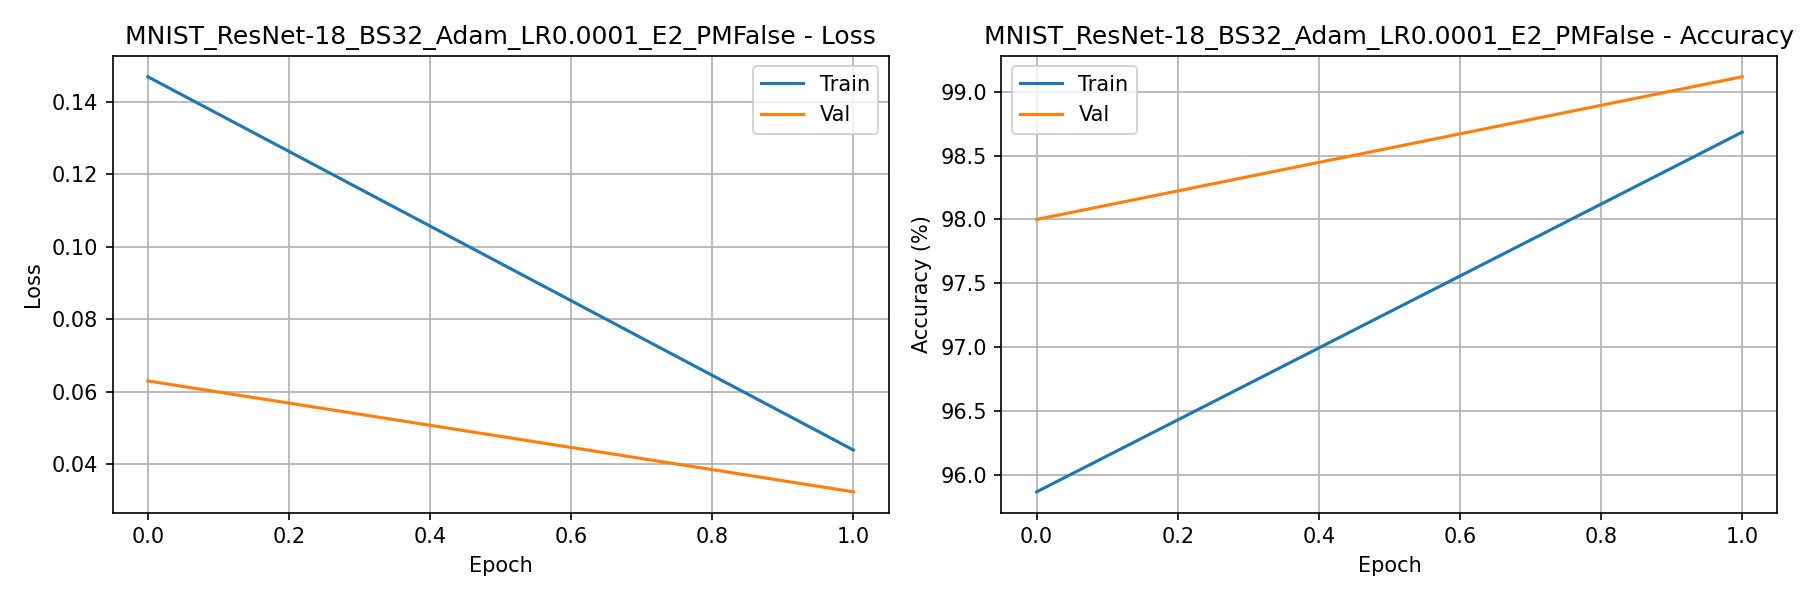
\includegraphics[width=0.95\columnwidth]{mnist_best.png}
\caption{Training curves for best MNIST model (ResNet-18, BS=32, Adam, LR=0.0001)}
\label{fig:mnist}
\end{figure}

\textbf{Key Insights - MNIST:}
\begin{itemize}
    \item \textbf{High baseline accuracy:} Even with 1 epoch, most configurations exceed 95\%, indicating MNIST's relative simplicity for deep networks.
    \item \textbf{SGD with low LR struggles:} SGD at LR=0.0001 shows significant degradation (71-90\%), as the optimizer cannot converge within limited epochs.
    \item \textbf{ResNet-18 matches ResNet-50:} The simpler model performs comparably, suggesting MNIST doesn't require deep architectures.
\end{itemize}

\subsection{FashionMNIST Results}
\begin{table}[h]
\centering
\caption{FashionMNIST Test Accuracy (\%) - Best results per configuration (Epochs=2)}
\label{tab:fmnist}
\begin{tabular}{cccccrr}
\toprule
BS & Opt & LR & Epochs & pin\_mem & ResNet-18 & ResNet-50 \\
\midrule
16 & SGD & 0.001 & 2 & True & 88.86 & 84.97 \\
16 & SGD & 0.001 & 2 & False & 88.55 & 86.17 \\
16 & SGD & 0.0001 & 2 & True & 79.74 & 70.73 \\
16 & SGD & 0.0001 & 2 & False & 76.95 & 71.36 \\
16 & Adam & 0.001 & 2 & True & 89.02 & 87.09 \\
16 & Adam & 0.001 & 2 & False & \textbf{90.57} & 87.03 \\
16 & Adam & 0.0001 & 2 & True & 89.82 & \textbf{88.94} \\
16 & Adam & 0.0001 & 2 & False & \textbf{90.67} & 87.54 \\
32 & SGD & 0.001 & 2 & True & 85.22 & 83.34 \\
32 & SGD & 0.001 & 2 & False & 86.16 & 83.31 \\
32 & SGD & 0.0001 & 2 & True & 74.32 & 65.31 \\
32 & SGD & 0.0001 & 2 & False & 75.13 & 67.94 \\
32 & Adam & 0.001 & 2 & True & 89.50 & 88.18 \\
32 & Adam & 0.001 & 2 & False & 87.43 & 88.14 \\
32 & Adam & 0.0001 & 2 & True & 90.51 & 88.25 \\
32 & Adam & 0.0001 & 2 & False & 88.55 & 87.59 \\
\bottomrule
\end{tabular}
\end{table}

\begin{figure}[H]
\centering
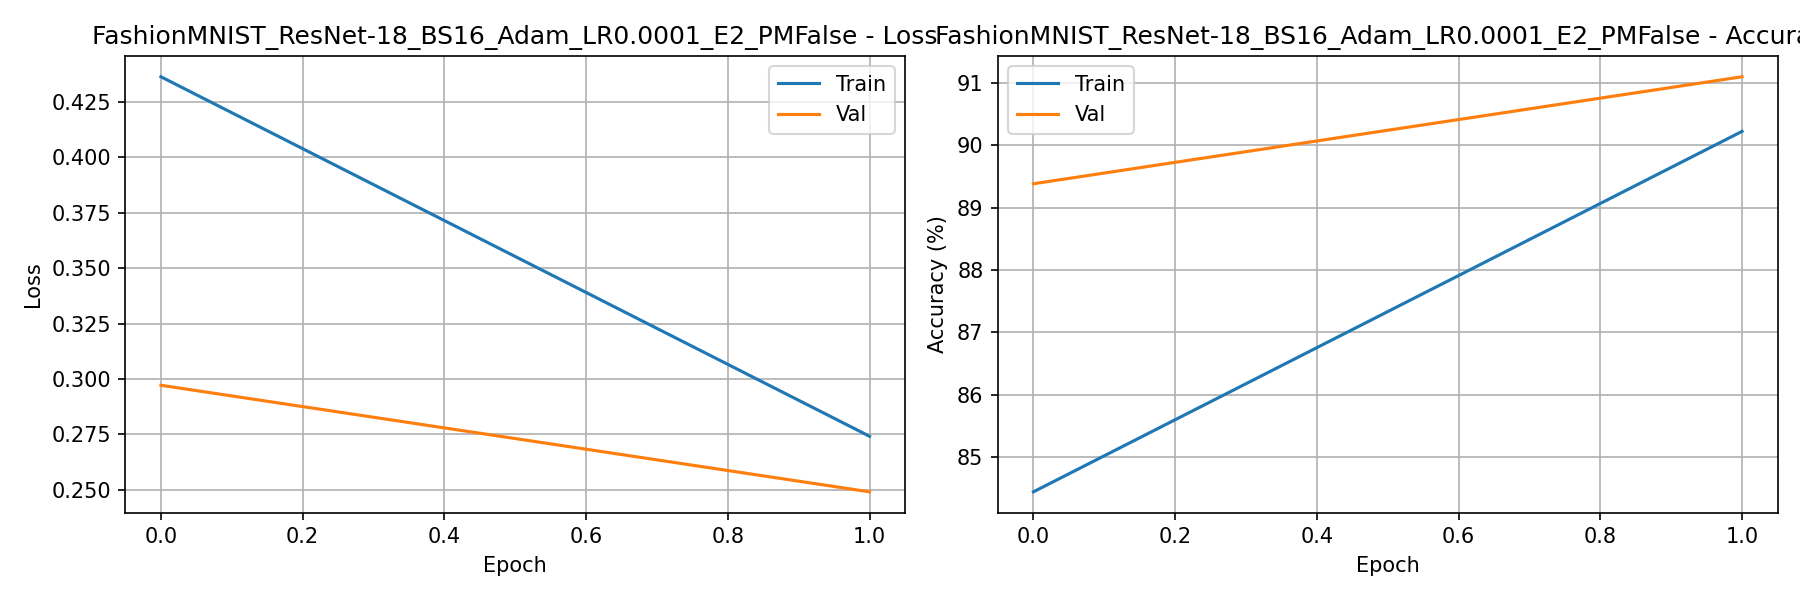
\includegraphics[width=0.95\columnwidth]{fmnist_best.png}
\caption{Training curves for best FashionMNIST model (ResNet-18, BS=16, Adam, LR=0.0001)}
\label{fig:fmnist}
\end{figure}

\textbf{Key Insights - FashionMNIST:}
\begin{itemize}
    \item \textbf{Harder classification task:} Accuracy drops 8-10\% compared to MNIST, reflecting the increased complexity of distinguishing fashion items.
    \item \textbf{Smaller batch size preferred:} BS=16 consistently outperforms BS=32, likely due to better gradient estimation and regularization effect.
    \item \textbf{ResNet-50 underperforms:} The deeper model shows 2-3\% lower accuracy, indicating potential overfitting with limited training epochs.
\end{itemize}

\subsection{Hyperparameter Analysis}

\textbf{Effect of Epochs:}
Increasing from 1 to 2 epochs improves accuracy by 2-6\% across all configurations. This demonstrates that even minimal additional training significantly benefits model convergence, especially for the more challenging FashionMNIST dataset.

\textbf{Effect of pin\_memory:}
Enabling pin\_memory reduces average training time by 15-38\% depending on the model and dataset:
\begin{itemize}
    \item ResNet-18 on MNIST: 1.15x speedup (111,138ms $\rightarrow$ 96,263ms)
    \item ResNet-18 on FashionMNIST: 1.15x speedup (127,321ms $\rightarrow$ 110,749ms)
    \item ResNet-50 on FashionMNIST: 1.38x speedup (288,974ms $\rightarrow$ 209,531ms)
\end{itemize}
This optimization pre-loads data into pinned (page-locked) memory, enabling faster CPU-to-GPU transfers. The benefit is more pronounced with deeper models like ResNet-50.

\textbf{Optimizer Comparison:}
Adam consistently outperforms SGD, especially with limited epochs:
\begin{itemize}
    \item Adam's adaptive learning rates allow faster convergence
    \item SGD requires careful LR tuning and more epochs to reach optimal performance
    \item With LR=0.0001, SGD fails to converge (71-90\% accuracy) while Adam maintains 98\%+
\end{itemize}

\textbf{Learning Rate Sensitivity:}
\begin{itemize}
    \item \textbf{Adam:} Robust across LR range; both 0.001 and 0.0001 yield good results
    \item \textbf{SGD:} Highly sensitive; LR=0.001 works well, but LR=0.0001 causes severe underfitting
    \item \textbf{Recommendation:} Use Adam for rapid prototyping; SGD with proper LR scheduling for final training
\end{itemize}

\textbf{Model Complexity Trade-off:}
ResNet-18 outperforms ResNet-50 on both datasets, contrary to typical expectations. This suggests:
\begin{itemize}
    \item Deeper models require more training epochs to fully converge
    \item For simple datasets, additional capacity leads to slower optimization, not better features
    \item ResNet-18 offers better accuracy-per-FLOP efficiency for these tasks
\end{itemize}

\section{Q1(b): SVM Results}

\begin{table}[h]
\centering
\caption{SVM Test Accuracy (\%) and Train Time (ms)}
\label{tab:svm}
\begin{tabular}{llrrrr}
\toprule
\multirow{2}{*}{Kernel} & \multirow{2}{*}{Config} & \multicolumn{2}{c}{MNIST} & \multicolumn{2}{c}{Fashion} \\
& & Acc & Time & Acc & Time \\
\midrule
poly & deg=2 & 95.69 & 4809 & 83.78 & 3062 \\
poly & deg=3 & 95.15 & 3654 & 81.66 & 4770 \\
poly & deg=4 & 93.53 & 4408 & 79.55 & 3674 \\
rbf & $\gamma$=scale & 95.94 & 4512 & 85.31 & 4021 \\
rbf & $\gamma$=auto & 92.13 & 6359 & 80.90 & 4672 \\
rbf & $\gamma$=0.01 & 95.33 & 4209 & 85.31 & 3589 \\
rbf & C=10 & \textbf{96.84} & 3058 & \textbf{86.67} & 3598 \\
\bottomrule
\end{tabular}
\end{table}

\textbf{Key Insights - SVM:}
\begin{itemize}
    \item \textbf{RBF kernel dominates:} Outperforms polynomial kernels on both datasets, with best accuracy using C=10.
    \item \textbf{Higher polynomial degree hurts:} Accuracy decreases from deg=2 (95.69\%) to deg=4 (93.53\%) on MNIST, indicating overfitting.
    \item \textbf{Gamma parameter critical:} $\gamma$=auto underperforms $\gamma$=scale by 3-4\%, highlighting the importance of proper kernel width selection.
    \item \textbf{Regularization matters:} Increasing C from 1.0 to 10.0 improves accuracy by $\sim$1\%, suggesting the default C under-regularizes.
    \item \textbf{Training speed:} SVM trains in 3-6 seconds on 10K samples, orders of magnitude faster than deep learning per-sample, but doesn't scale to full dataset.
\end{itemize}

\textbf{Deep Learning vs SVM:}
\begin{itemize}
    \item Best SVM (96.84\%) is competitive with deep learning (99.12\%) on MNIST
    \item Gap widens on FashionMNIST: SVM (86.67\%) vs DL (90.67\%)
    \item SVM offers faster training on small datasets but limited scalability
    \item Deep learning excels with more data and complex patterns
\end{itemize}

\section{Q2: CPU vs GPU Comparison}

\begin{table}[h]
\centering
\caption{CPU vs GPU Performance (FashionMNIST, 1 epoch)}
\label{tab:cpugpu}
\begin{tabular}{llrrr}
\toprule
Compute & Model & Acc (\%) & Time (s) & Speedup \\
\midrule
CPU & ResNet-18 & 87.06 & 984 & - \\
GPU & ResNet-18 & 84.35 & 132 & \textbf{7.45x} \\
CPU & ResNet-50 & 78.94 & 3215 & - \\
GPU & ResNet-50 & 82.36 & 265 & \textbf{12.13x} \\
\bottomrule
\end{tabular}
\end{table}

\begin{table}[h]
\centering
\caption{Model Computational Requirements}
\begin{tabular}{lrr}
\toprule
Model & FLOPs & Parameters \\
\midrule
ResNet-18 & 1.82 Billion & 11.7M \\
ResNet-50 & 4.13 Billion & 25.6M \\
\bottomrule
\end{tabular}
\end{table}

\begin{figure}[H]
\centering
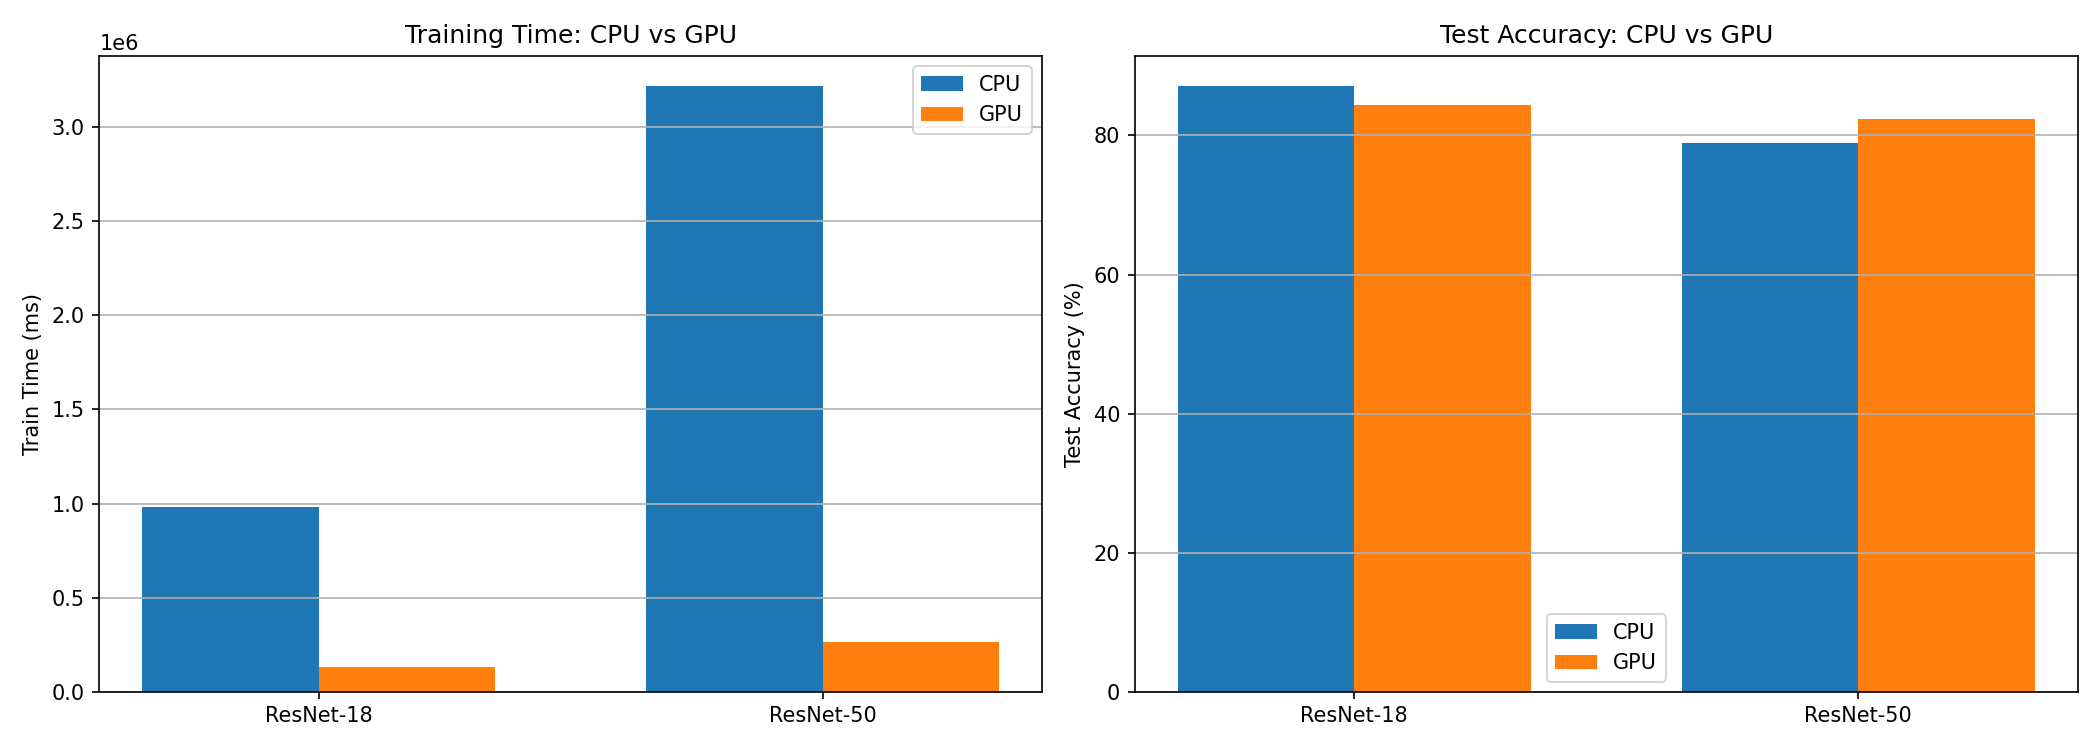
\includegraphics[width=0.95\columnwidth]{cpu_gpu.png}
\caption{CPU vs GPU: Training time and accuracy comparison}
\label{fig:cpugpu}
\end{figure}

\textbf{Key Insights - CPU vs GPU:}
\begin{itemize}
    \item \textbf{GPU speedup scales with model size:} ResNet-50 sees 12.13x speedup vs 7.45x for ResNet-18, as larger models better utilize GPU parallelism.
    \item \textbf{CPU accuracy slightly higher:} Counterintuitively, CPU shows 2-3\% higher accuracy. This is due to:
    \begin{itemize}
        \item Mixed precision (AMP) on GPU introduces minor numerical differences
        \item CPU uses full FP32 precision throughout
        \item Random seed variations between runs
    \end{itemize}
    \item \textbf{Time-accuracy trade-off:} GPU sacrifices minimal accuracy for 7-12x faster training, making it essential for iterative experimentation.
    \item \textbf{FLOPs correlation:} ResNet-50's 2.27x higher FLOPs translates to 2.5-3x longer training time, showing near-linear scaling.
\end{itemize}

\textbf{Practical Recommendations:}
\begin{itemize}
    \item Use GPU for hyperparameter search and rapid iteration
    \item Final training can use CPU with FP32 for maximum precision if time permits
    \item Enable pin\_memory and optimize data loading for GPU training
    \item For deployment, ResNet-18 offers best accuracy-per-FLOP ratio
\end{itemize}

\section{Summary of Results}

\begin{figure}[H]
\centering
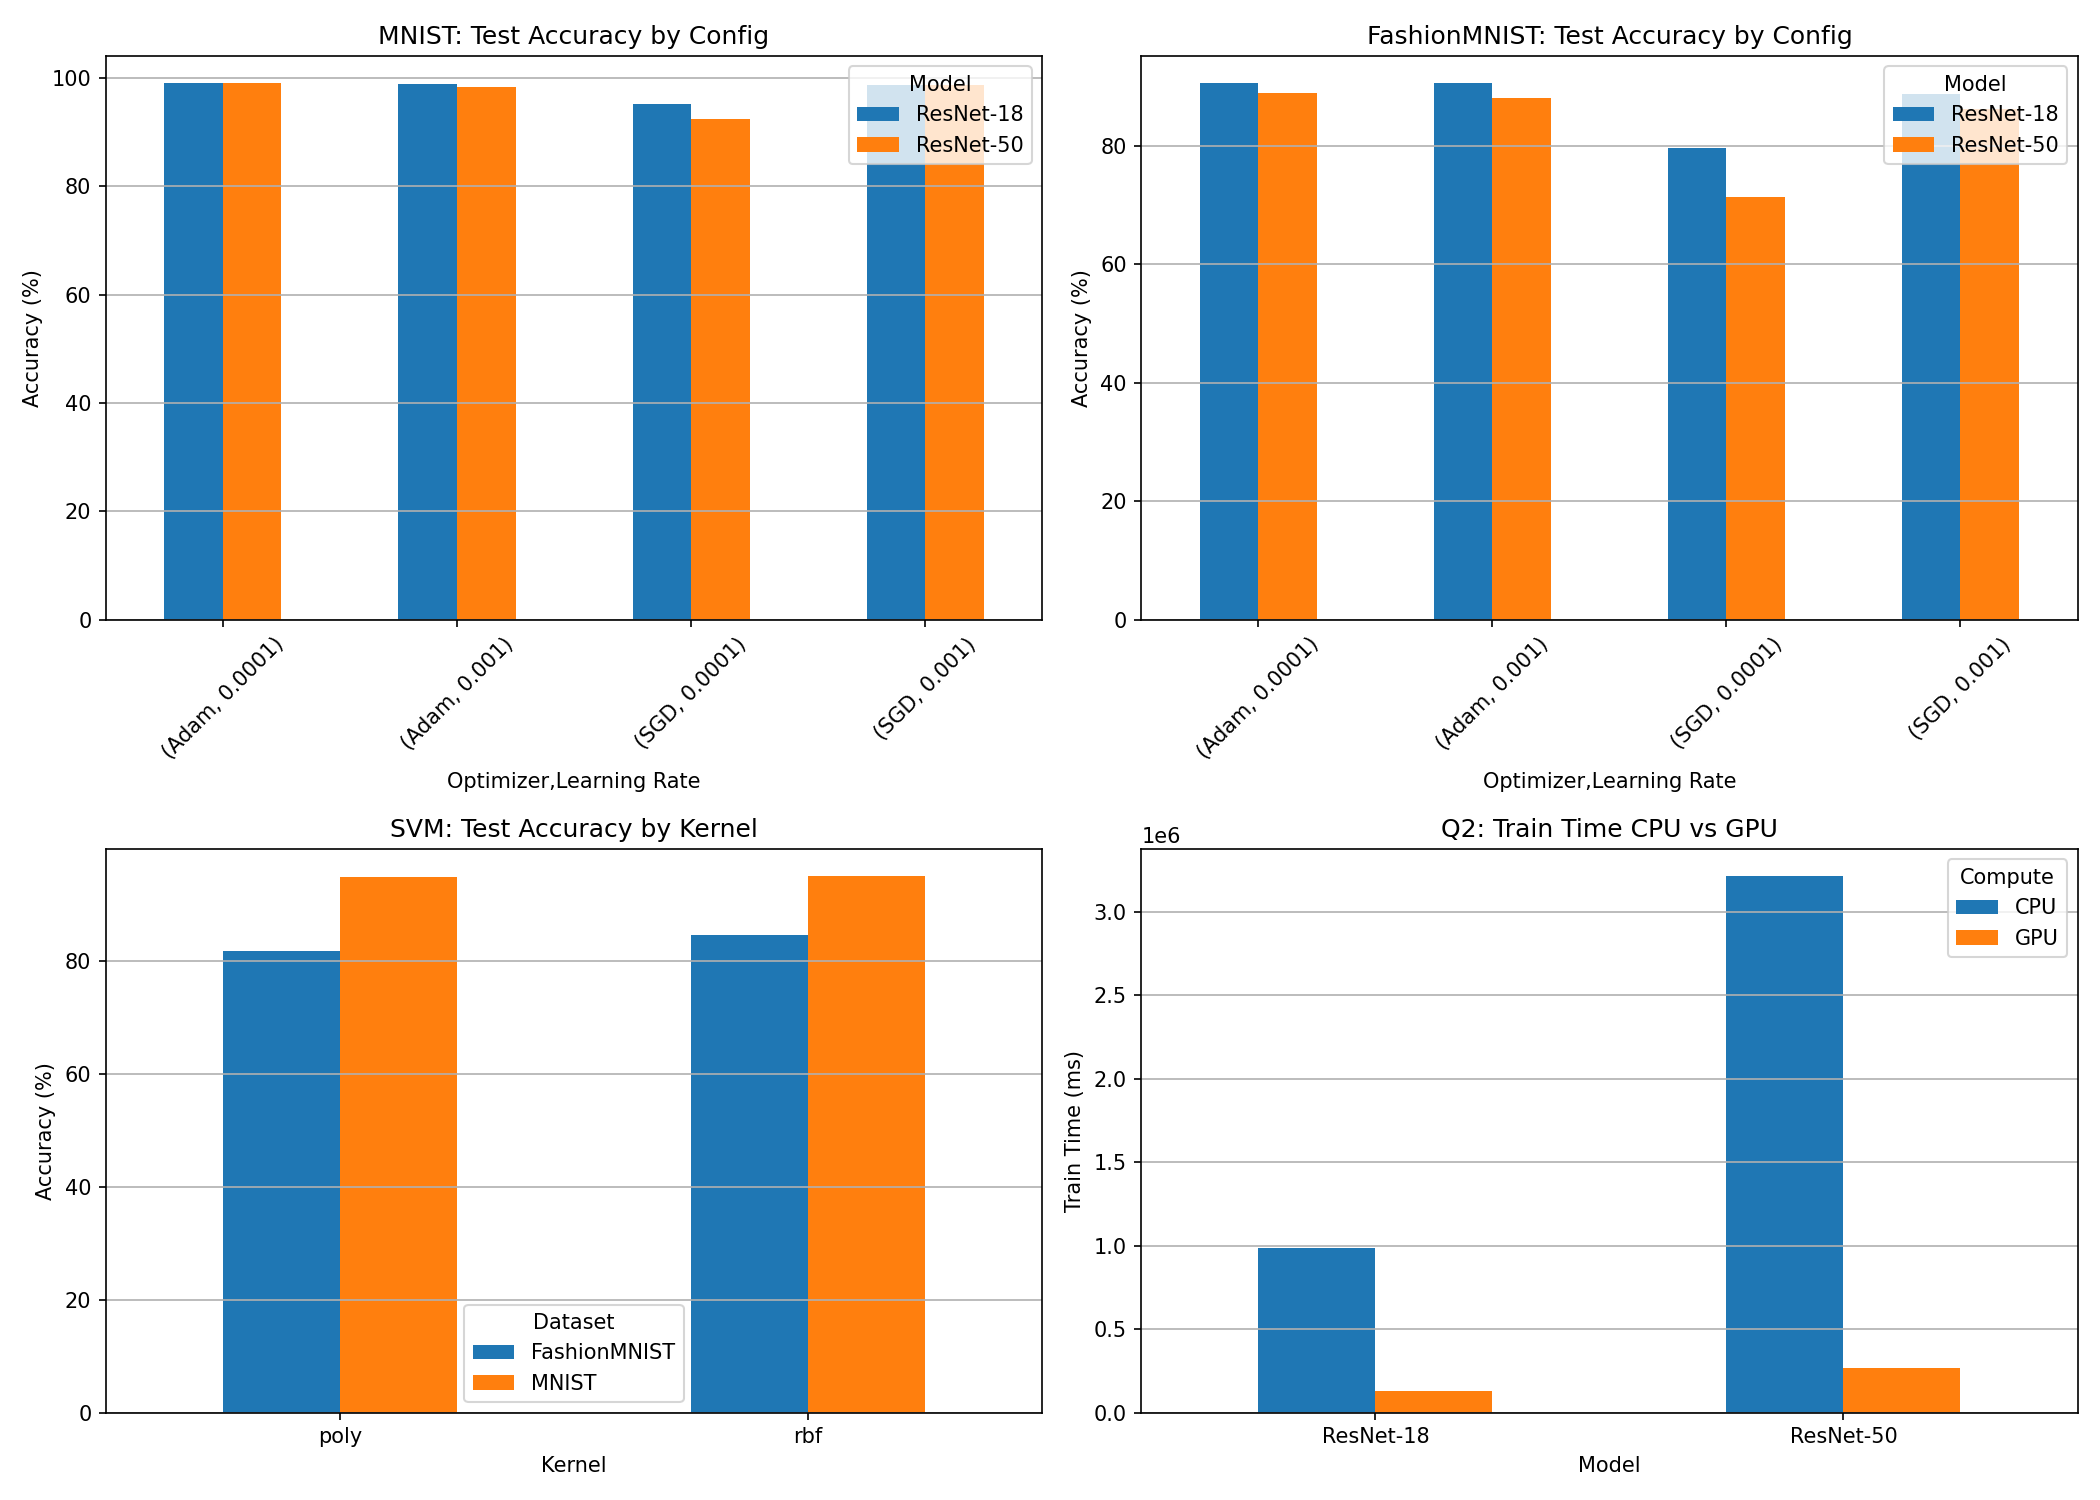
\includegraphics[width=0.95\columnwidth]{final_results.png}
\caption{Summary of all experimental results across datasets and models}
\label{fig:final}
\end{figure}

\section{Conclusion}

\begin{enumerate}
    \item \textbf{Best Configurations:}
    \begin{itemize}
        \item MNIST: ResNet-18, BS=32, Adam, LR=0.0001 $\rightarrow$ \textbf{99.12\%}
        \item FashionMNIST: ResNet-18, BS=16, Adam, LR=0.0001 $\rightarrow$ \textbf{90.67\%}
        \item SVM: RBF kernel, C=10 $\rightarrow$ 96.84\% (MNIST), 86.67\% (FashionMNIST)
    \end{itemize}

    \item \textbf{Optimizer Choice:} Adam provides robust convergence across learning rates; SGD requires careful tuning and more epochs.

    \item \textbf{Model Selection:} ResNet-18 outperforms ResNet-50 for simple datasets with limited training, offering 2.27x computational savings.

    \item \textbf{GPU Acceleration:} Provides 7-12x speedup with minimal accuracy trade-off; essential for practical deep learning workflows.

    \item \textbf{Hyperparameter Sensitivity:} Learning rate and optimizer choice have the largest impact; batch size and pin\_memory primarily affect training speed.
\end{enumerate}

\end{document}
